\documentclass[master.tex]{subfiles}

\chapter{Project Plan}

\section{Preliminary}

The work that has been done so far is the specification (see \autoref{chap:specification}) of phometa and examples (see \autoref{chap:examples}) to show that this specification is good enough.

I have started some part of implementation, however there is a major change on specification during Autumn term and it is quite hard to update it. So I decide to redo most of work anyway. \autoref{fig:preliminary-dir} \autoref{fig:preliminary-code} \autoref{fig:preliminary-screen} show an implementation that has been done so far.

\begin{figure}[H]
    \centering
    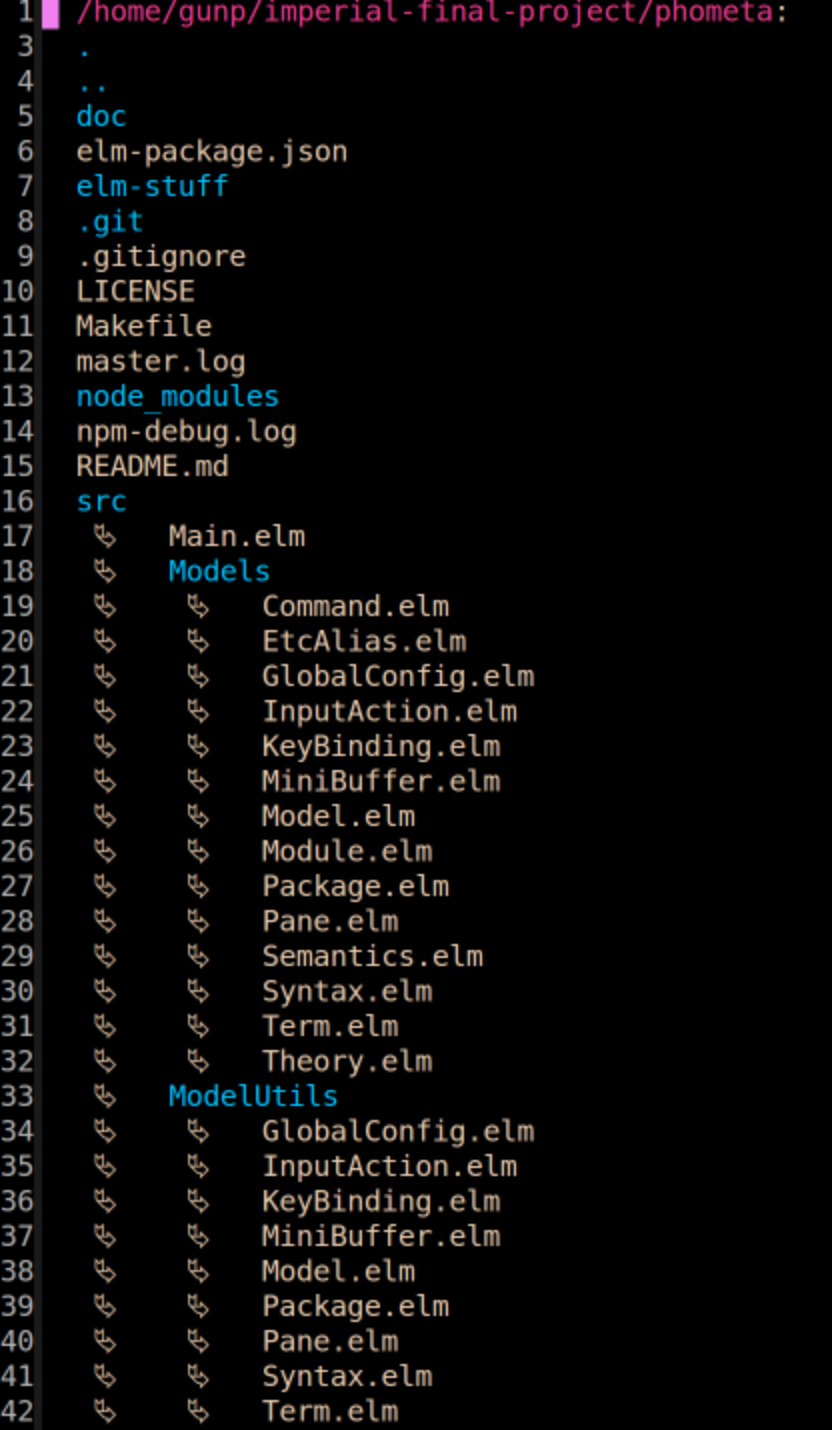
\includegraphics[width=0.3\textwidth]{preliminary-dir1}
    \hspace{1cm}
    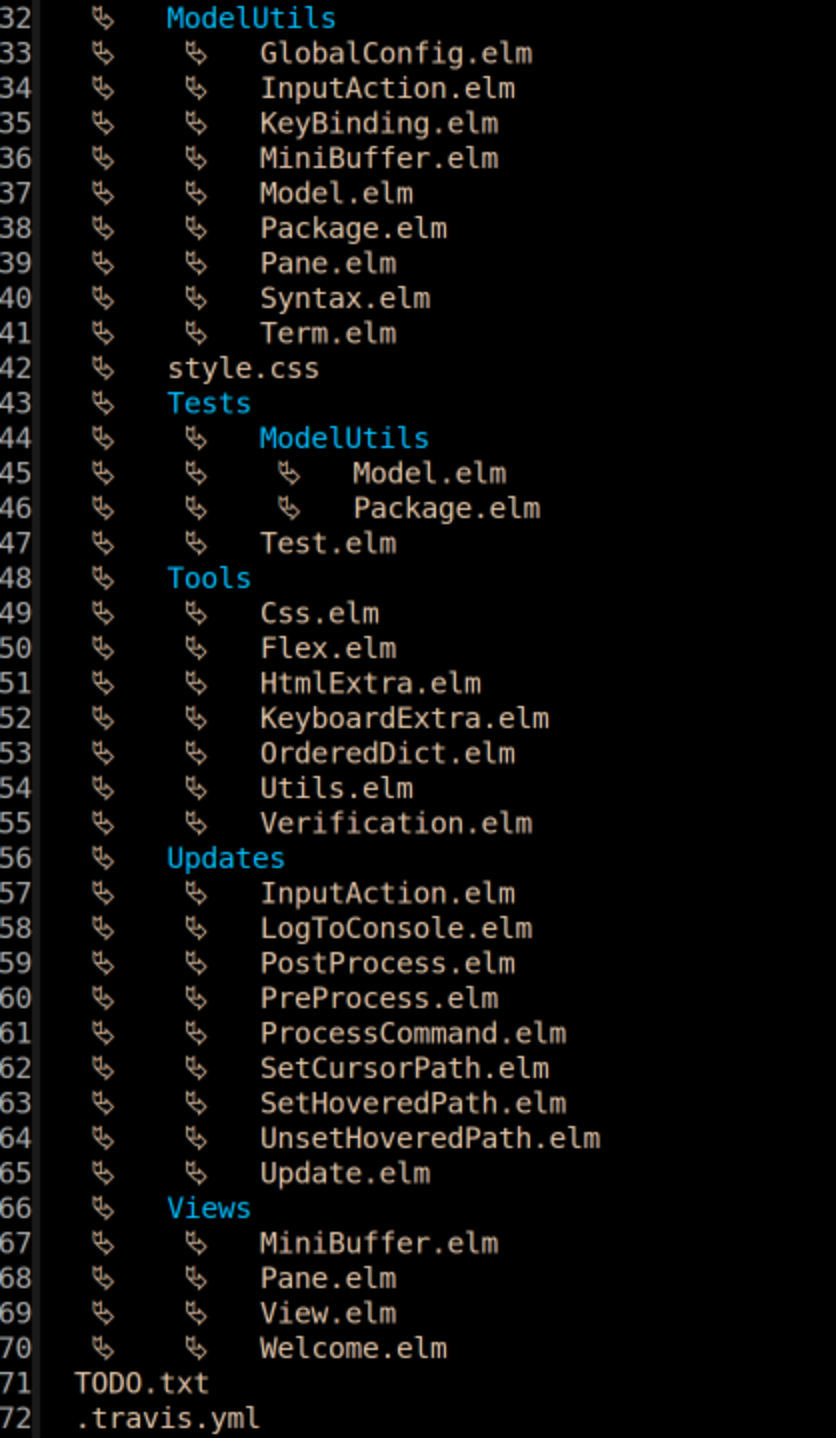
\includegraphics[width=0.3\textwidth]{preliminary-dir2}
    \caption{Directory of preliminary work.}
\label{fig:preliminary-dir}
\end{figure}

\begin{figure}[H]
    \centering
    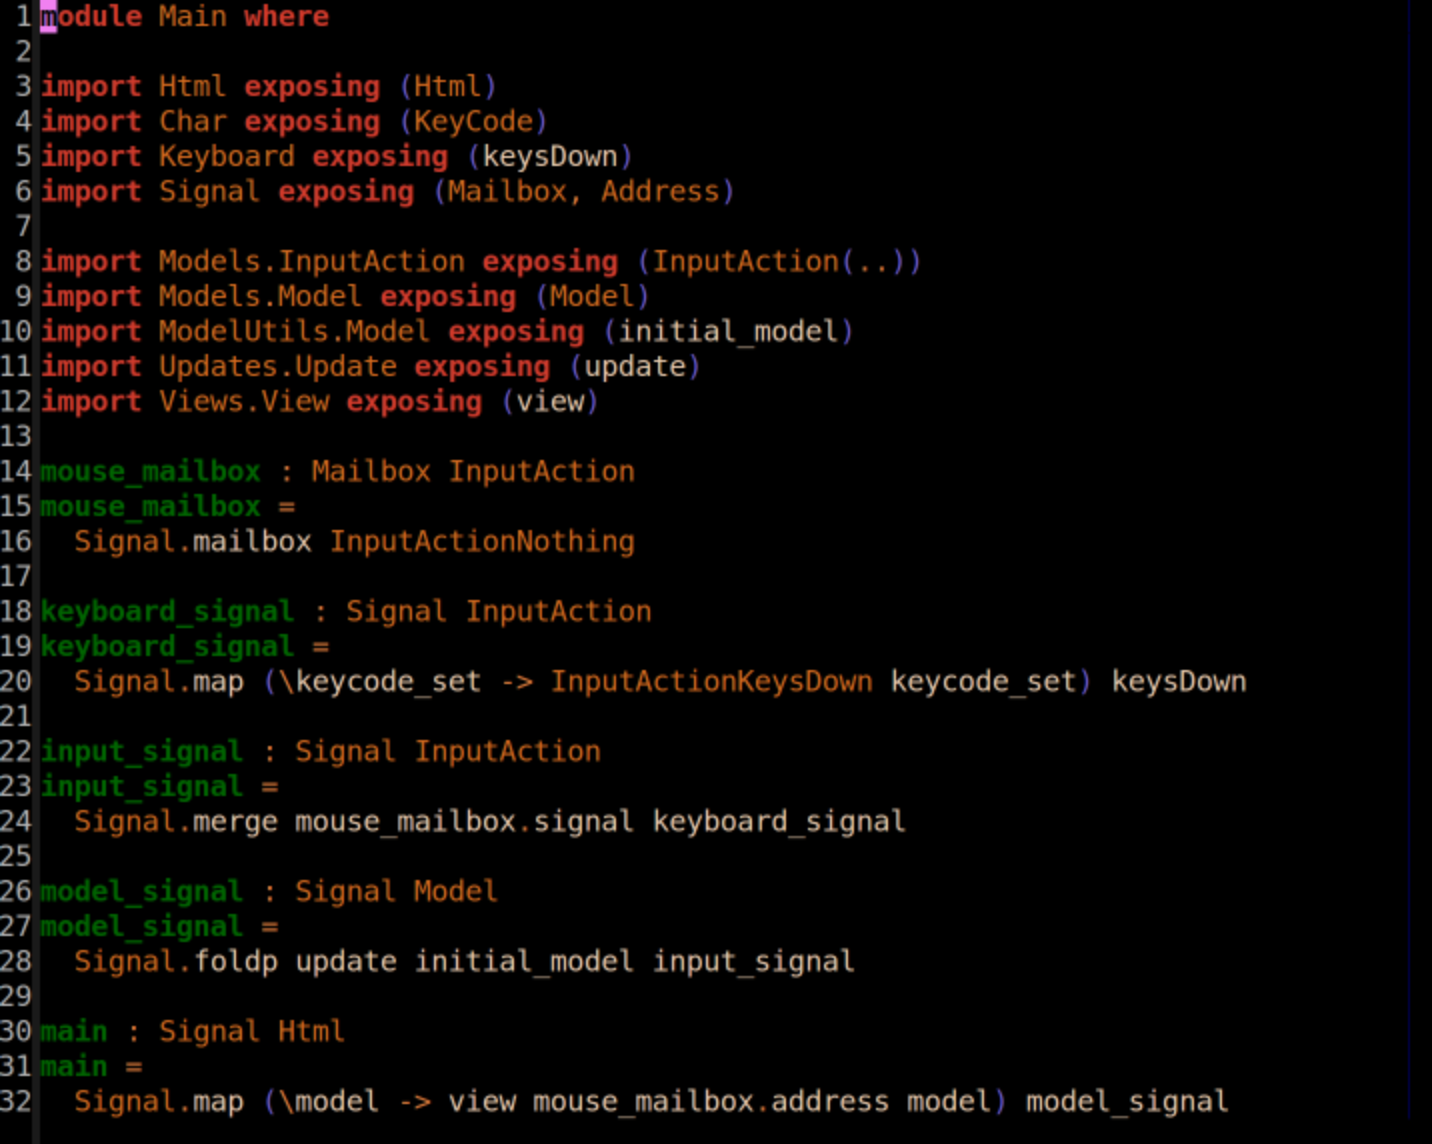
\includegraphics[width=0.6\textwidth]{preliminary-code}
    \caption{Code of some part of preliminary work.}
\label{fig:preliminary-code}
\end{figure}

\begin{figure}[H]
    \centering
    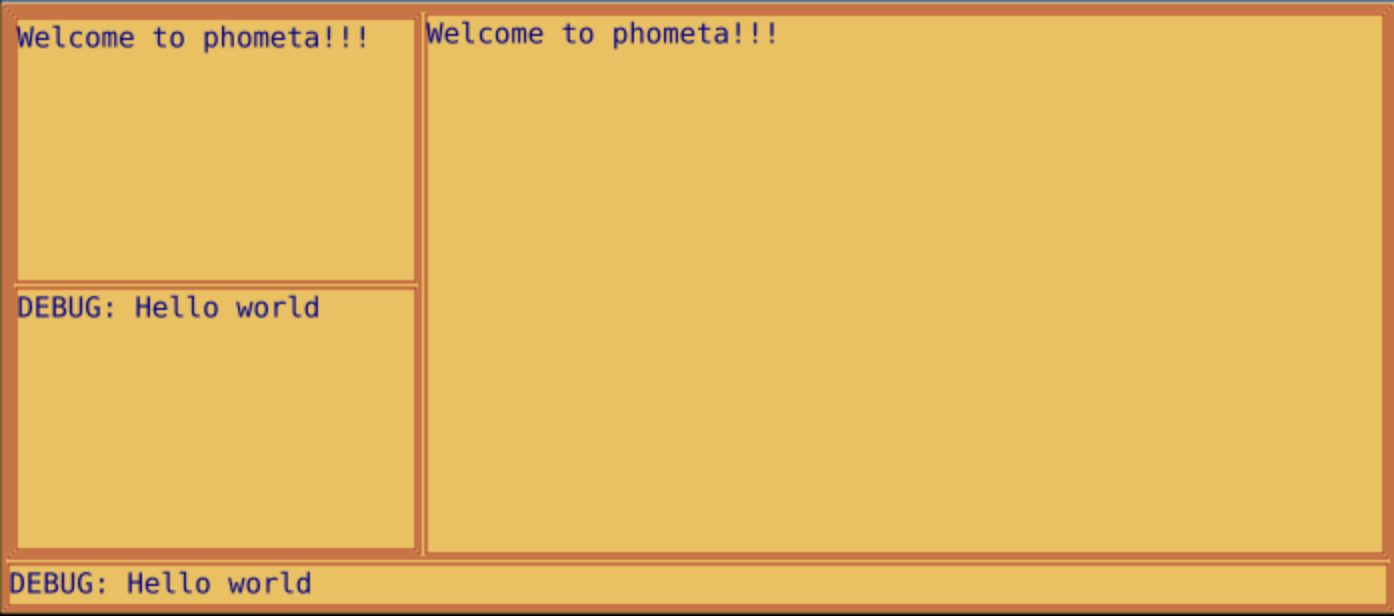
\includegraphics[width=0.6\textwidth]{preliminary-screen}
    \caption{Screen shot of preliminary work.}
\label{fig:preliminary-screen}
\end{figure}

\section{Risk management}
Once I decide to do this project, I was aware that it could be risky. So I started to do background research since $3^{rd}$ year industial placement. This gave me an opportunity to work on this project without pressure which result in better specification and guarantee this would not be a bad project.

However, There is something I miss as well, I didn't keep track of what I have read so far which make it harder to actually write down the background section.

Lastly, Some spare-time is left in planning. If there are some part that take longer than I expect, I could use this spare-time to finish it without postpone the entire plan.

\section{Project Timeline}

\paragraph{June 2015} Started to do research on the project. Mostly did tutorials and practiced on Coq to get better understanding about proof assistant.

\paragraph{July 2015 --- The end of summer} Sketched the specification of phometa structure and tried to implement it (using Elm programming language).
This was a lot harder than I expect, and I needed to change the specification serveral times. The most time-consuming part was Elm technical problem.

\paragraph{Autumn term} As design always changing, I try to focus on one particular formal system which was propositional logic (along with sequential calculus). This result in a huge change of specification which made the draft of implementation very hard to refactor. I also started to write draft of report including chapter on specification, and examples.

\paragraph{Chrismas break} Spent most of time to prepare for PhD application, hence, didn't work on the project seriously.

\paragraph{Spring term, week 2 --- 3} Writing up chapters on Introduction, Background, and Project plan.

\paragraph{Spring term, week 4} Refactor existing draft of implementation, the project workflow including Emacs setup, Makefile, newer version of Elm and continuous integration should work without any error.

\paragraph{Spring term, week 5} Update ``Model'' part of Model-Controller-View (MCV) to current specification.

Also the ``Model'' part of Model-Controller-View (MCV) should be almost complete.

\paragraph{Spring term, week 6} Implement module system and project explorer. \kOpen\ and \kComment\ node should work as well.

\paragraph{Spring term, week 7} Implement \kInductive\ \kGrammar\ node and ``term'' input method.

\paragraph{Spring term, week 8 --- 9} Implement \kInference\ \kRule\ node, \kTheorem\ (excluding buildin rules) node and its input method. By this time, minimum working version of phometa is done.

\paragraph{Spring term, week 10 --- 11} Spend all time with revision and final exam.

\paragraph{24 --- 31 March} Spare week. If the minimum working version hasn't been complete, so finish it by these weeks. Otherwise, write some part of the final report.

\paragraph{1 --- 8 April} Easter holiday.

\paragraph{9 --- 12 April} Implement \kDefinition\ and its detail including \kMatch, \kLet\ \kBe.

\paragraph{12 --- 17 April} Implement \kSequence\ and \kLiteral\ \kGrammar. And its input method.

\paragraph{17 --- 22 April} Implement all builtin rules.

\paragraph{Summer term, early week 1} Implement \kCompound\ \kRule\ and \kAlias\

\paragraph{Summer term, late week 1} Spare time for unfinished work, otherwise write more on report. By this time all specification should have been completed.

\paragraph{Summer term, week 2} Implement famous formal systems as examples that will be included in the final product

\paragraph{Summer term, week 3} Extension, if get any idea.

\paragraph{Summer term, week 4 --- 5} Project evaluation.

\paragraph{Summer term, week 6 --- the firnal report due} Working on report, attempt to write full reference to phometa as appendiex.


\section{Features to implement}

\subsection{foldable node and subnode (extension, do it later)}

We should allow user to fold/unfold any node which will hide/show all of content except header of the node. This also apply to subnodes (things that has thick vertical bar as indentation) by click on the vertical bar, everything that is indented will be hide and leave a button in front of subnode header for unfold later.

\subsection{hide/show root grmmar by default, popup subterm grammar when  grammar when hover underline container}

When we create a (root) term, usually we ask user to specify its grammar, and it will show there on the the same line with root term. This might look complicate and unreadable when dealing with complex term. So, user can set in ``preference page'' to hide grammar of root term by default (but it will ask grammar when root term created anyway). This might not confuse user since they always be able to hover the root term (specifically on the main underline) to see grammar of that root term. Moreover, this technique also apply to sub  apply to subterm, so whenever they hover the underline of subterm, the corresponding grammar will be shown.

\subsection{manage nodes inside project explorer}

We will list all nodes for each module on project explorer. So we can create/delete/reorder nodes inside project explorer directly. Moreover, if we click on a node, it will show just that node on main panel, this allow us to focus on complex node (of course, we can click on a module to show all nodes inside it on main panel, however, this doesn't work for packages).

\subsection{variable resolution inside theorem}

For example, in type system, sometime we construct a derivation tree in order to get type of particular term. This can be done inside phometa as well, by construct a normal judgement and leave the type as variable e.g. \bat{\pvar{$\Gamma$} \pifmt{$\vdash$} \pvar{$\phi$} \pifmt{:} \pvar{A}} you can see that we leave type as \pvar{A}. Then build its derivation tree by \kTheorem, at some point it will hit a rule involve inference on \pvar{A} (term deconstruction). Let say \pvar{A} get deconstruct into \bat{\pvar{B} \pifmt{$\rightarrow$} \pvar{C}} (of course, user need to write ``B'' and ``C'' to get \pvar{B} and \pvar{C} during using particular rule) then every \pvar{A} appear inside that theorem will be replace by \bat{\pvar{B} \pifmt{$\rightarrow$} \pvar{C}} as we desire. Eventually, the type of main is in final form. Please note that this works in general not just type theory case.

\subsection{construct a new (sub) term by copying an existing (sub) term (extension, do it later)}

On the actual proof, there will a complex term that needed to be modified on the
small portion and left the rest untouch. Constructing this modified term from
the scratch would be tedious. So we can just copy the old term then modify it.
Recall that we need to press ``c'' for inductive/literal/sequence/dictionary
construction, ``v'' for variable, ``d'' for definition, ``a'' for alias. Here
inside term hole, we just type ``m'' then we just click the underline of that
term, then it will check grammar of both term which needed to be matched then we
get that term. Then for the part that we want to modify we just click ``h'' on
underline of target subterm, this would replace hold to it then you can
construct that subterm. Once you finish it just press ``q'', so phometa we check
this new term against rule if it is in theorem or something else depent on the
place of that term.

%%% Local Variables:
%%% mode: latex
%%% TeX-master: "master"
%%% End:
